\chapter{Global methods for design and verification}\label{section:global_methods}

In the previous chapter, we introduced local gradient-based optimization methods for design, both using standard optimization and adversarial verification-guided optimization. However, there are three notable drawbacks to these approaches.

\begin{enumerate}
    \item \textbf{Risk of local minima: } Local gradient-based optimizers are greedy and prone to getting stuck in local minima. This risk is particularly important in verification use cases, since converging to a set of exogenous parameters that is far from the true worst-case could lead the system designer to falsely believe that their system is safe.
    \item \textbf{Lack of diversity in adversarial examples: } When verifying a system, it is important to consider a diverse set of failure modes. However, optimization-based approaches have difficulty balancing exploration with exploitation, often simply converging to the nearest local optimum.
    \item \textbf{Sensitivity to gradient quality: } Many robotic systems, particularly those involving contact or vision, have dynamics that are not differentiable everywhere, as we assumed in the previous chapter. Even when these dynamics are smoothed, there are still regions where the gradients can be poorly conditioned (i.e. arbitrarily large) or flat, which will cause a gradient-based optimizer to diverge or get stuck.
\end{enumerate}

In this chapter, we will address all of these drawbacks by re-framing the optimization and verification problems as Bayesian inference problems, which we will then solve using gradient-accelerated Markov Chain Monte Carlo (MCMC) methods. We will demonstrate empirically how this Bayesian inference framework provides improved performance (in both convergence speed and solution quality) over both gradient-based and gradient-free optimization methods. The results in this chapter represent ongoing work that has been submitted to NeurIPS 2023 and CoRL 2023.

% Motivate this section by framing the limitations of local methods in the context of an engineer exploring the design space.

% Introduce the capabilities that we want to provide for an engineer: predicting the different ways in which an autonomous system might fail

% Once we have the failure modes, updating the design to mitigate those failure modes.

% Provide a motivating example - SCOPF (others?)

\subsection{From optimization to inference}

To motivate the switch from optimization to inference, consider the toy example of optimizing the cost landscape shown on the left in Fig.~\ref{global:fig:toy_example}. This cost function has local minima at $x = -0.544$ and $x = 0.919$ (the latter represents the true global minimum). If initialized with $x < 0$, a local gradient-based optimizer will naturally converge to the sub-optimal local minimum at $x = -0.544$ (the square in Fig.~\ref{global:fig:toy_example}), missing the global minimum (marked by a circle). We can see this behavior in Fig.~\ref{global:fig:toy_example_convergence}, which plots the convergence of gradient-based optimization with 5 different random starting positions $x\sim\cN(-1.5, 0.1)$. All 5 runs converge to the suboptimal local minimum at $x = -0.544$.

To avoid getting stuck in this local minimum, we can convert the optimization $\argmin_x U(x)$ into the inference problem of sampling from the unnormalized probability density $x \sim p(x) \propto e^{-U(x)}$. This distribution is shown on the right in Fig.~\ref{global:fig:toy_example}. We can see that the distribution is bimodal, with a peak at the suboptimal local minimum and a larger peak at the global minimum. By sampling from this distribution, we can find the global minimum with high probability (this is the so-called \textit{Optimization as Inference} approach~\cite{maSamplingCanBe2019,levineReinforcementLearningControl2018a}). In practice, we can approximately sample from this distribution using Markov Chain Monte Carlo (MCMC) methods, which we will discuss in more detail shortly. The benefit of these methods is that they balance exploring different regions of the distribution with exploiting high-likelihood areas; we can see this behavior in Fig.~\ref{global:fig:toy_example_convergence}, which shows the convergence of Metropolis-adjusted Langevin (MALA) MCMC, a gradient-based inference method, on the same cost landscape over 5 different random seeds. MALA is able to converge to the global minimum with high probability, while gradient-based optimization gets stuck in the local minimum.

\begin{figure}[tb]
    \centering
    \includegraphics[width=0.6\linewidth]{images/global_methods/sampling_as_optimization.png}
    \caption{Left: a simple bimodal cost landscape $U(x) = x^4 - 0.5 x^3 - x^2$, with a locally optimal solution at $x\approx -0.544$ and a global optimum at $x\approx 0.919$. Right: the corresponding unnormalized likelihood $p(x) \propto e^{-U(x)}$, showing samples drawn from this distribution (black dots) and the average of 100 samples (red dot).}
    \label{global:fig:toy_example}
\end{figure}

\begin{figure}[tb]
    \centering
    \includegraphics[width=0.6\linewidth]{images/global_methods/double_well_gd_mala.png}
    \caption{Convergence of gradient-based optimization and inference (Metropolis-adjusted Langevin) on the double-well cost landscape from Fig.~\ref{global:fig:toy_example}, showing how the optimization method gets stuck in a local minimum while the inference method is able to escape and find the global minimum.}
    \label{global:fig:toy_example_convergence}
\end{figure}

A wide variety of MCMC algorithms exist to sample from arbitrary non-normalized probability distributions~\cite{geyerIntroductionMarkovChain2011}; common variants include Random-walk Metropolis-Hastings (RMH), Hamiltonian Monte Carlo (HMC), unadjusted Langevin (ULA), and MALA. RMH is gradient-free, while HMC, ULA, and MALA are both gradient-based. MALA, which can be seen as a single-step version of HMC, is outlined in Algorithm~\ref{ch6:alg:mala}. Like all MCMC algorithms, it defines a Markov chain with a transition rule designed to preserve the so-called detailed balance condition, which ensures that the stationary distribution of the Markov chain is the same as the target density (see~\cite{geyerIntroductionMarkovChain2011,aiama} for a more complete introduction). MALA defines a transition rule that begins by proposing a candidate new state in line~\ref{ch6:alg:mala:step} by combining a gradient-driven drift term with a Gaussian diffusion term. The candidate state is accepted with probability $P_{accept}$ in line~\ref{ch6:alg:mala:mh}, which is proportional to the ratio of the target density at the candidate state and the current state. If the candidate state is accepted, it becomes the new current state; otherwise, the current state is repeated. The algorithm is run for $K$ steps, and the final state is returned as the sample from the target density.

\begin{algorithm}
    \caption{Metropolis-adjusted Langevin algorithm (MALA,~\cite{maSamplingCanBe2019,robertsLangevinDiffusionsMetropolisHastings2002})\label{ch6:alg:mala}}
    \DontPrintSemicolon
    \KwInput{Initial $x_0$, steps $K$, stepsize $\tau$, density $p(x)$.}
    \KwOutput{A sample drawn from $p(x)$.}
    \For{$i = 1, \ldots, K$}
    {
    Sample $\eta \sim \cN(0, 2\tau I)$ \Comment{Gaussian noise}\;
    $x_{i+1} \gets x_i + \tau \nabla \log p(x_i) + \eta$ \Comment{Propose next state}\;\label{ch6:alg:mala:step}
    $P_{accept} \gets \frac{p(x_{i+1}) e^{-||x_i - x_{i+1} - \tau \nabla \log p(x_{i+1})||^2 / (4\tau)}}{p(x_{i}) e^{-||x_{i+1} - x_{i} - \tau \nabla \log p(x_{i})||^2 / (4\tau)}}$ \;
    With probability $1 - \min(1, P_{accept})$:
    \hspace{2em}$x_{i+1} \gets x_{i}$ \Comment{Accept/reject proposal}\;\label{ch6:alg:mala:mh}
    }
    \KwRet{$x_K$}
\end{algorithm}

We have shown how transitioning from gradient-based optimization to inference (in particular, gradient-based inference using MALA) addresses the first drawback identified at the start of this section (the risk of getting stuck in local minima). Next, we will show how gradient-based inference also addresses the other two drawbacks (the difficulty of sampling diverse failure modes and sensitivity to gradient quality).

\paragraph{Sampling diverse failure modes} MCMC sampling methods provide a principled means for balancing exploration and exploitation, and so they are well-suited to problems with multiple modes (particularly when the modes are close together in the search space). However, although MCMC methods enjoy good asymptotic guarantees, including ergodicity and convergence to the target distribution in the inifinite-sample limit, any finite-sample implementation of MCMC will struggle to explore well-separated modes of a highly multi-modal target distribution (any finite MCMC run will be biased towards the modes near its initialization). A family of algorithms known as sequential Monte Carlo (SMC) algorithms exist to solve this problem by smoothly interpolating between a sequence of distributions, starting from a simple distribution (e.g., a Gaussian) and ending at the target distribution~\cite{chopinIntroductionSequentialMonte2020}. SMC algorithms are particularly useful for inference problems with multiple modes, since they can be used to sample from the target distribution in a way that is less biased by the initialization. In the following section, we will discuss how SMC can be applied to sample diverse failure modes for practical autonomous system verification problems.

\paragraph{Sensitivity to gradient quality} Prior work~\cite{suhDifferentiableSimulatorsGive2022} identifies the ballistic optimization problem shown in Fig.~\ref{global:fig:ballistic} as a challenging test case for gradient-based optimizers, since the flat region and discontinuities represent a challenge for gradient-based optimizers. We implement this example using a differentiable contact simulator does not apply any smoothing; so the objective function is discontinuous and has large regions where the gradients are zero. Despite these challenging features, MALA is able to find the global optimum, as shown on the left in Fig.~\ref{global:fig:ballistic_convergence}.

The authors of~\cite{suhDifferentiableSimulatorsGive2022} argue that these discontinuities and flat regions should favor a gradient-free solution method over one that uses gradients, and so it is worth comparing gradient-based inference (MALA) with gradient-free methods like RMH. We can see in Fig.~\ref{global:fig:ballistic_convergence} that on low-dimensional versions of this problem, the gradient-free and gradient-based inference algorithms perform similarly; however, on higher-dimensional problems (which we create by running multiple instances in parallel and concatenating the decision variables for each instance), there is a clear advantage for the gradient-based method.

We attribute this improved performance to three factors. First, the Gaussian diffision term in the MALA proposal allows it to explore the flat region of the cost landscape and eventually find the optimal solution. Second, the accept/reject step provides some robustness to stiff or inaccurate gradients; if a bad gradient causes MALA to propose a state with much higher cost (lower likelihood), then it will likely reject that proposal and try again. Third, the gradient-based drift term in the proposal provides a valuable heuristic for exploring high-dimensional space, where the exponentially decreased volume of the region around the optimal solution makes it difficult to explore using gradient-free methods.

\begin{figure}[t]
    \centering
    \begin{subfigure}[t]{0.6\linewidth}
        \centering
        
\includegraphics[width=\linewidth]{images/global_methods/ballistic.png}
    \end{subfigure}
    \begin{subfigure}[t]{0.3\linewidth}
        \centering
        \includegraphics[width=\linewidth]{images/global_methods/ballistic_cost.png}
    \end{subfigure}%
    \caption{Left: the ballistic optimization problem from~\cite{suhDifferentiableSimulatorsGive2022}. Right: the corresponding cost landscape.}
    \label{global:fig:ballistic}
\end{figure}

\begin{figure}[tb]
    \centering
    \begin{subfigure}[t]{0.24\linewidth}
        \centering
        \includegraphics[width=\linewidth]{images/global_methods/ballistic_1.png}
    \end{subfigure}
    \begin{subfigure}[t]{0.24\linewidth}
        \centering
        \includegraphics[width=\linewidth]{images/global_methods/ballistic_10.png}
    \end{subfigure}
    \begin{subfigure}[t]{0.24\linewidth}
        \centering
        \includegraphics[width=\linewidth]{images/global_methods/ballistic_100.png}
    \end{subfigure}
    \begin{subfigure}[t]{0.24\linewidth}
        \centering
        \includegraphics[width=\linewidth]{images/global_methods/ballistic_1000.png}
    \end{subfigure}
    \caption{Convergence of gradient-based optimization (gradient descent), gradient-based inference (MALA), and gradient-free inference (RMH) on the ballistic cost landscape from Fig.~\ref{global:fig:toy_example}, showing how the inference methods are robust to flat and discontinuous regions of the cost function, and how gradient-based methods excel on high-dimensional problems. From left to right: 1-, 10-, 100-, and 1000-dimensional versions of the problem.}
    \label{global:fig:ballistic_convergence}
\end{figure}

\subsection{Sampling and repairing diverse failure modes}

Now that we have motivated the switch from optimization to inference, we will reframe the verification and verification-guided design problems in~\eqref{ch5:eq:verification} and~\eqref{ch5:eq:verification_guided_design_minmax} as inference problems, then demonstrate how we can used gradient-accelerated MCMC sampling (i.e. MALA) to efficiently sample diverse failure modes.

Recall that verification, or \textit{failure prediction}, entails finding exogenous parameters $y^*$ that, for some given $x$, lead to a high cost. To ensure that the predicted failures are plausible, it is important to balance maximizing cost with choosing values for $y^*$ with high prior likelihood. To achieve this balance, we define the metric of \textit{risk-adjusted cost}
\begin{align}
    J_r(x, y) = J \circ S(x, y) + \log p_{y, 0}(y)
\end{align}
where $\circ$ denotes function composition. Failure prediction is thus the problem of finding parameters $y^*$ that lead to a high risk-adjusted cost; moreover, since it is likely that $J_r$ will have multiple local minima with respect to $y$ (i.e. multiple likely failure modes), we wish to sample a set $\set{y^*_1, \ldots, y^*_{n_y}}$ of such high risk-adjusted cost failures. To generate this set, we convert the deterministic optimization problem $y^* = \argmax_y J_r(x, y)$ to the problem of sampling from the unnormalized probability distribution
\begin{align}
    y^* \sim p(y^* | x) \propto p_{y, 0}(y^*) e^{J \circ S(x, y^*)} \label{ch6:eq:prediction_distribution}
\end{align}

Similarly, we can reframe verification-guided design optimization, or \textit{failure mitigation}, as an inference problem. To do so, we assume that, just as there is a prior over exogenous factors $p_{0, y}$, there is also a prior over designs $p_{0, x}$ that reflects the constraints and the designer's prior beliefs about the design space (e.g. assigning zero prior probability to infeasible designs). Failure mitigation then seeks to find design parameters $x^*$ that both have high prior likelihood (thus respecting the designer's prior beliefs about the design space) and results in a low cost across a range of anticipated failure modes. We might frame this as an optimization problem, $x^* = \min_x \left[ \expectation_y J(x, y) + \log p_{x, 0}(x) \right]$ taking the expectation over the likely failure modes distribution~\eqref{ch6:eq:prediction_distribution}, but for the reasons discussed above it is more productive to frame this as a probabilistic sampling problem akin to the one used for failure prediction. To this end, we frame the problem of mitigating a set of failure modes $y^*_1, \ldots, y^*_{n_y}$ as the problem of sampling from the unnormalized distribution
\begin{align}
    x^* \sim p(x^* | y^*_1, \ldots, y^*_{n_y}) \propto p_{x, 0}(x^*) e^{-\sum_{i} J\circ S(x^*, y^*_i) / n_y} \label{ch6:eq:mitigation_distribution}
\end{align}

Using this framework, we can replace the alternating min/max optimization presented in Chapter~\ref{section:local_methods} with a novel adversarial sampling algorithm that alternates between sampling a more robust design and sampling a more likely set of failure modes. This algorithm is presented in Algorithm~\ref{ch6:alg:smc}. It is important to note that this is not the first work to make the connection between MCMC sampling and verification, as~\cite{zhouRoCUSRobotController2021} uses gradient-free sampling to for failure mode prediction and~\cite{sinhaNeuralBridgeSampling2020} uses gradient-based sampling for failure probability analysis, but this is the first work (to our knowledge) that uses sampling to solve adversarial design optimization optimization problems.

Our algorithm (detailed in Algorithm~\ref{ch6:alg:smc}) proceeds in the style of a sequential Monte Carlo algorithm~\cite{chopinIntroductionSequentialMonte2020}. We begin by initializing $n_y$ potential failure modes and $n_x$ candidate designs sampled from their respective prior distributions. Then, in each of $K$ rounds, we first sample $n_x$ new candidate designs from distribution~\eqref{ch6:eq:mitigation_distribution} to mitigate the current set of predicted failure modes. We then select the design that performs best against all currently-predicted failure modes and sample $n_y$ new sets of exogenous parameters (each representing a potential failure mode) from distribution~\eqref{ch6:eq:prediction_distribution} to degrade the performance of the selected design. To sample from distributions~\eqref{ch6:eq:prediction_distribution} and~\eqref{ch6:eq:mitigation_distribution}, we use $n_x$ and $n_y$ parallel executions of the Metropolis-adjusted Langevin algorithm (MALA,~\cite{robertsLangevinDiffusionsMetropolisHastings2002}), a gradient-based MCMC sampling algorithm detailed in Algorithm~\ref{ch6:alg:mala}. In order to handle potential multimodality in the design and failure space, we include optional tempering to interpolate between the prior and target distributions, following~\cite{chopinIntroductionSequentialMonte2020}.

\begin{algorithm}
    \caption{Failure prediction and mitigation using gradient-based sampling\label{ch6:alg:smc}}
    \DontPrintSemicolon
    \KwInput{Design and failure population sizes $n_x$, $n_y$; rounds $K$; substeps $M$; stepsize $\tau$; tempering schedule $\lambda_1, \ldots, \lambda_K$.}
    \KwOutput{Robust design $x^*$ and a set of failures $\set{y_1^*, \ldots, y_{n_y}^*}$ with high risk-adjusted cost.}
    Initialize candidate designs $[x]_0 = \set{x_1, \ldots, x_{n_x}}_0$ sampled from $p_{x, 0}(x)$\;
    Initialize candidate failures $[y]_0 = \set{y_1, \ldots, y_{n_y}}_0$ sampled from $p_{y, 0}(y)$\;
    \For{$i = 1, \ldots, K$}
    {
        $p_{x, i}(x) := p_{x, 0}(x)e^{-\lambda_k / n_y \sum_{y \in [y]_{i-1}} J\circ S(x, y)}$ \Comment{Update designs using predicted failures}\;
        $[x]_i \gets \text{MALA}([x]_{i-1}, M, \tau, p_{x, i})$\;
        $p_{y, i}(y) := p_{y, 0}(y)e^{\lambda_k\min_{x \in [x]_{i-1}} J\circ S(x, y)}$ \Comment{Update failure predictions for new best design}\;
        $[y]_i \gets \text{MALA}([y]_{i-1}, K, \tau, p_{y, i})$\;
    }
    $x^* \gets \argmax_{x \in [x]_{N}} p_{x, i}(x)$ \Comment{Choose best design}\;
    \KwRet{$x^*$, $[y]_K$}
\end{algorithm}

Before moving on to our experimental results, we must discuss a few practical and theoretical aspects of Algorithm~\ref{ch6:alg:smc}. On a theoretical level, the use of MALA (or any MCMC algorithm) to sample from a distribution is sound so long as the resulting Markov chain is ergodic and satisfies detailed balance~\cite{aiama}. The use of Gaussian noise ensures ergodicity (since there is non-zero probability of transitioning between any two feasible states), while the Metropolis-Hastings accept/reject step in Line~\ref{ch6:alg:mala:mh} of Algorithm~\ref{ch6:alg:mala} enforces detailed balance. Unfortunately, there can be a large practical gap between the asymptotic guarantees provided by these conditions and practically acceptable performance.

First, if the target distribution is multimodal and the modes are well-separated, then MCMC algorithms may be slow to move between modes and will yield a biased sampling distribution with any finite number of steps. To mitigate this effect when the target distributions~\eqref{ch6:eq:prediction_distribution} and~\eqref{ch6:eq:mitigation_distribution} are highly multimodal, we include a tempering schedule $0 \leq \lambda_1 \leq \ldots \leq \lambda_K \leq 1$ to interpolate between the prior and target distributions and run multiple MALA instances in parallel from different initial conditions. We find empirically that tempering is not always needed, but we include it for completeness.

The second potential practical challenge arises from the continuity and differentiability (or lack thereof) of the simulator and cost function $J \circ S$. Although MALA remains sound so long as the target distribution is continuously differentiable almost everywhere (i.e. discontinuous or non-differentiable on a set of measure zero), in practice performance may suffer when the target distribution has large discontinuities (it may take an unacceptably long time to accept a move across a discontinuity). As with the problems caused by multimodality, this issues can also be mitigated using of tempering.

The final practical consideration is that although the stochasticity in our sampling-based approach can help us explore the design and failure spaces, we incur a degree of sub-optimality as a result. To reduce this sub-optimality, it is possible to ``quench'' the solution provided by our method by turning off the stochasticity on the last few rounds and executing simple gradient descent (e.g. using MALA for the first 90 rounds and then gradient descent on the last 10 rounds). In practice, we find that quenching can noticeably improve the final cost without compromising the diversity of predicted failure modes.

% Motivation: how to close the design-verification feedback loop.

% Convert min-max optimization from previous section to inference problem.

% Introduce sequential MCMC algorithm for solving this problem.

\subsubsection{Case study: robust generation dispatch for secure power networks}

To see this approach in practice, consider the motivating example of controlling an electric power transmission network subject to failures in transmission lines. Two simple networks (the IEEE 14- and 57-node test system) are shown in Fig.~\ref{global:fig:networks}. The goal in this problem is to find control inputs (power injection and voltage at each generator, and power demand at each load) that ensure that the voltage seen by each load is stable, even in the event of transmission outages (which we model using a bimodal distribution for the admittance of each line). The simulator models the AC power flow through this network, and the cost function penalizes excessively high or low voltages or any violation of rated generator capacities. More details on this motivating example is provided in the appendix.

Given a transmission network, the so-called \textit{security-constrained optimal power flow problem} (or SCOPF~\cite{capitanescuStateoftheartChallengesFuture2011}) is the problem of scheduling generator setpoints and power demand from loads to minimize the economic cost of generation and ensure that the network operates safely (satisfying voltage and maximum power constraints) in the event of transmission line outages. The design parameters $x = (P_g, |V|_g, P_l, Q_l)$ include the real power injection $P_g$ and AC voltage amplitude $|V|_g$ at each generator in the network and the real and reactive power draws at each load $P_l, Q_l$; all of these parameters are subject to minimum and maximum bounds that we model using a uniform prior distribution $p_{x, 0}$. The exogenous parameters are the state $y_i \in \R$ of each transmission line in the network; the admittance of each line is given by $\sigma(y_i) Y_{i, nom}$ where $\sigma$ is the sigmoid function and $Y_{i, nom}$ is the nominal admittance of the line. The prior distribution $p_{y, 0}$ is an independent Gaussian for each line with a mean chosen so that $\int_{-\infty}^0 p_{y_i, 0}(y_i) dy_i$ is equal to the likelihood of any individual line failing (e.g. as specified by the manufacturer; we use $0.05$ in our experiments). The simulator $S$ solves the nonlinear AC power flow equations~\cite{cainHistoryOptimalPower2012} to determine the state of the network, and the cost function combines the economic cost of generation $c_g$ (a quadratic function of $P_g, P_l, Q_l$) with the total violation of constraints on generator capacities, load requirements, and voltage amplitudes:
\begin{align}
    J = & c_g + v(P_g, P_{g, min}, P_{g, max}) + v(Q_g, Q_{g, min}, Q_{g, max}) \\
        & + v(P_l, P_{l, min}, P_{l, max}) + v(Q_l, Q_{l, min}, Q_{l, max})     \\
        & + v(|V|, |V|_{min}, |V|_{max}) \label{eq:scopf_cost}
\end{align}
where $v(x, x_{min}, x_{max}) = L\pn{[x - x_{max}]_+ + [x_{min} - x]_+}$, $L$ is a penalty coefficient ($L=100$ in our experiments), and $[\circ]_+ = \max(\circ, 0)$ is a hinge loss.

Efficient solutions to SCOPF are the subject of active research~\cite{capitanescuStateoftheartChallengesFuture2011} and an ongoing competition run by the U.S. Department of Energy~\cite{u.s.departmentofenergyGridOptimizationCompetition}. In addition to its potential economic and environmental impact~\cite{cainHistoryOptimalPower2012}, SCOPF is also a useful benchmark problem for 3 reasons: 1) it is highly non-convex, 2) it has a large space of possible failures, and 3) it can be applied to networks of different sizes to test an algorithm's scalability. In our case, the 14-bus network has 32 design parameters and 20 exogenous parameters, while the 57-bus network has 98 design parameters and 80 exogenous parameters.

\begin{figure}[tb]
    \centering
    \begin{subfigure}[t]{0.4\linewidth}
        \centering
        \includegraphics[width=\linewidth]{images/global_methods/base_14_bus.png}
    \end{subfigure}
    \begin{subfigure}[t]{0.4\linewidth}
        \centering
        \includegraphics[width=\linewidth]{images/global_methods/IEEE57.png}
    \end{subfigure}%
    \caption{Example 14- and 57-bus electricity transmission networks~\cite{illinoiscenterforasmarterelectricgridIEEE57BusSystem}.}
    \label{global:fig:networks}
\end{figure}

We can compare our approach quantitatively with the following baselines. \textbf{GD}: solving the adversarial optimization problem $\min_x \max_y J_r(x, y)$ by alternating between optimizing a population of $n_x$ designs and $n_y$ failure modes using local gradient descent. GD is analogous to the methods proposed in~\cite{dontiAdversariallyRobustLearning2021} and in the work in the previous chapter~\cite{dawsonRobustCounterexampleguidedOptimization2022}, modified to provide a fair comparison by using populations of design and exogenous parameters rather than single examples (we intend this baseline to also be representative of a broad class of gradient-based falsifiers~\cite{xuAdversarialAttacksDefenses2020}). \textbf{RMH}: implements Alg.~\ref{ch6:alg:smc} using gradient-free Metropolis-Hastings MCMC with a Gaussian kernel instead of MALA. This baseline represents the straightforward extension of gradient-free failure prediction techniques like ROCUS~\cite{zhouRoCUSRobotController2021} to solve the mitigation problem as well. In addition to these benchmarks, we also include \textbf{GD-NoAdv} to demonstrate what happens when we run \textbf{GD} without updating the exogenous parameters. GD-NoAdv does not represent the state of the art but instead illustrates the benefit of intelligently predicting failure modes rather than relying on vanilla domain randomization.

We implement our method and all baselines in Python using the JAX framework for automatic differentiation and just-in-time compilation. Experiments were run on a laptop with 8 GB of RAM, an 8-core Intel i7-865U CPU running at \SI{1.8}{GHz}, and no GPU. To ensure a fair comparison, all techniques are run with the same population sizes $n_x = n_y = 10$ and total sample budget $KM(n_x + n_y) = 2\times 10^4$ ($K = 100$, $M = 10$); this sample budget was chosen to be large enough that all methods converged. After manual tuning, we found that a step size of $\tau = 10^{-2}$ was appropriate for the exogenous parameters, but $\tau = 10^{-6}$ was required for the design parameters to ensure stability of gradient-based methods. We found that tempering was not required for this problem ($\lambda_i = 1$). For our method, we quench during the final 10 rounds.

We will first compare these methods based on the quality of the solutions they produce, and then on the the speed with which they converge to an optimized design.

\paragraph{Solution quality} To compare the quality of these methods' solutions, we use each method to optimize $n_x = 10$ candidate designs and predict $n_y=10$ failure modes with high risk-adjusted cost. We then select the design that achieves the highest likelihood according to Eq.~\eqref{ch6:eq:mitigation_distribution}, then use one additional round to sample new failure modes that attack the chosen design. The maximum cost across these final predicted failure modes provides a measure of each algorithm's confidence in its solution. We then compare the performance on these predicted failure modes to the maximum cost observed on a test set of $10^6$ exogenous parameters sampled randomly from the prior $p_{y, 0}$. Fig.~\ref{global:fig:14_bus_comparison} (top) shows the predicted and observed costs for each method on the IEEE 14-bus test case. The prediction-and-mitigation process took \SI{30.5}{s} for GD-NoAdv, \SI{61.5}{s} for GD, \SI{111.5}{s} for RMH, and \SI{141.7}{s} for our method (including the cost of JAX just-in-time compilation).

\begin{figure}[tb]
    \centering
    \includegraphics[width=0.45\linewidth]{images/global_methods/14_bus_comparison.png}
    \includegraphics[width=0.45\linewidth]{images/global_methods/57_bus_comparison.png}
    \caption{Comparison of our method with baselines for failure prediction and mitigation on a 14-bus (top) and 57-bus (bottom) power transmission network. Red markers show the maximum, mean, and minimum-cost failure modes predicted by each method after optimizing the design, while the box plot shows the distribution of costs on a test set of $10^6$ random failures. Our method not only successfully predicts failure modes that match the range of the empirical distribution, but it also finds a low-cost solution that is more robust than those found by other methods.}
    \label{global:fig:14_bus_comparison}
\end{figure}

We can assess these methods in two ways: by the quality of the optimized design and by the quality of the predicted failure cases. The two optimization-based methods, GD and GD-NoAdv, find solutions with the lowest best-case cost, but their solutions are not robust. Not only do these methods find solutions that are susceptible to a heavy tail of failures, but they are overconfident and fail to predict those failures (instead predicting that all 10 candidate failures will be successfully mitigated). In contrast, RMH is not overconfident (it successfully predicts failure modes that match the range of the empirical failure distribution), but it finds a solution that is 10 times costlier than that found by our method. Only our proposed method is able to find a robust, low-cost solution without being overconfident.

Once we have a robust design optimized using our method, we can examine the predicted failure modes to understand the remaining ways in which our design might fail. Of the 10 predicted failure modes, 4 include attacks on the transmission line connecting the generator at bus 7 to the rest of the network (this was the most commonly attacked line). Interestingly, of these 4 attacks, only one (shown in Fig.~\ref{global:fig:predicted_failure_modes}) is able to cause a violation of the voltage stability constraints. It is only by fully disconnecting the generator at bus 7 (dotted red line) and partially impairing the line between buses 1 and 4 (solid red; $15\%$ impairment) that we see the voltage drop at several buses (shown in orange). This information about potential failure modes can be very useful to system designers; in this example, the designer may choose to focus monitoring and infrastructure hardening efforts on the two affected lines.

\begin{figure}[tb]
    \centering
    \includegraphics[width=0.4\linewidth]{images/global_methods/predicted_failure_modes.png}
    \caption{The only predicted failure modes (of 10 candidates) that causes violation of voltage constraints on the 14-bus transmission network, using the optimized design found using our method. Fully disconnecting the generator at bus 7 (dotted red line) is not enough; other predicted failures include this outage but do not cause a constraint violation. It is only by additionally impairing the line between buses 1 and 4 that the voltage constraint is violated at the buses shown in orange.}
    \label{global:fig:predicted_failure_modes}
\end{figure}

To understand the scalability of our approach, we repeat this experiment on a larger 57-bus network with 80 transmission lines. All hyperparameters were the same except for the step size for exogenous parameters, which was reduced to $10^{-3}$. The results are shown in the bottom panel of Fig.~\ref{global:fig:14_bus_comparison}; we see that our approach continues to not only find a robust solutions (with a relatively light tail of failures) but also accurately predicts the range of possible failure modes (as opposed to RMH, which does not explore the full failure space in this case). Running GD-NoAdv on this example took \SI{406.2}{s}, GD took \SI{803.4}{s}, RMH took \SI{1002.3}{s}, and our method took \SI{1438.5}{s}.

\paragraph{Convergence rate} From comparing solution quality, there is a clear separation between the sampling- and optimization-based methods, with sampling able to find more robust designs and more accurately cover the range of possible failures (although our gradient-based approach finds higher-quality solutions in both the 14- and 57-node test cases). As a result, a natural question is how these two sampling-based methods compare in how quickly they converge.

To measure the relative convergence rate of RMH and our gradient-based method, we measure the average cost $J$ in each round across all candidate designs $[x]_i$ on a test set of 100 exogenous parameters sampled randomly from the prior distribution. The convergence of this test-set performance as a function of the number of sampling rounds is shown in Fig.~\ref{global:fig:training_curves} for both the 14- and 57-bus networks. These results show that our method converges much more quickly than gradient-free RMH, suggesting that the use of automatic differentiation provides a clear advantage.

\begin{figure}[tb]
    \centering
    \includegraphics[width=0.45\linewidth]{images/global_methods/14_bus_training_curves.png}
    \includegraphics[width=0.45\linewidth]{images/global_methods/57_bus_training_curves.png}
    \caption{Comparison of convergence rates of our method and a gradient-free sampling baseline on 14- (top) and 57-bus (bottom) power networks, showing average cost of 10 candidate designs on a test set of 100 random exogenous parameters. Our gradient-based method converges significantly faster than gradient-free RMH. The gradual increase in cost after convergence is likely due to distribution shift between the predicted failure modes and the prior distribution.}
    \label{global:fig:training_curves}
\end{figure}

\subsubsection{Case study: Vision-based control}

We have also applied our approach to problems involving visual feedback, implementing a differentiable rendering engine in JAX and applying the adversarial sampling approach from Algorithm~\ref{ch6:alg:smc}. We define a range of vision-based control tasks, from autonomous vehicle control to grasp keypoint prediction, as shown in Fig.~\ref{global:fig:vision_scenarios}. For each of these scenarios, a policy was pretrained using a traditional method (either PPO or behavior cloning), and then we apply our method to identify and repair failure modes.

Example failures for the drone and autonomous vehicle scenarios are shown on the left in Fig.~\ref{global:fig:repairs}, while the repaired policy is shown on the right for each case. We can see that some of the pretrained policies, such as for autonomous driving on a highway, are overly aggressive and prone to failures, while the repaired policy is much safer.

\begin{figure}
    \centering
    \includegraphics[width=\linewidth]{images/global_methods/all_scenarios.png}
    \caption{Environments for drone navigation, AV control, and household object manipulation. Inset: a robot's-eye-view of each scene rendered using our differentiable renderer.}\label{global:fig:vision_scenarios}
\end{figure}

\begin{figure}[t]
    \centering
    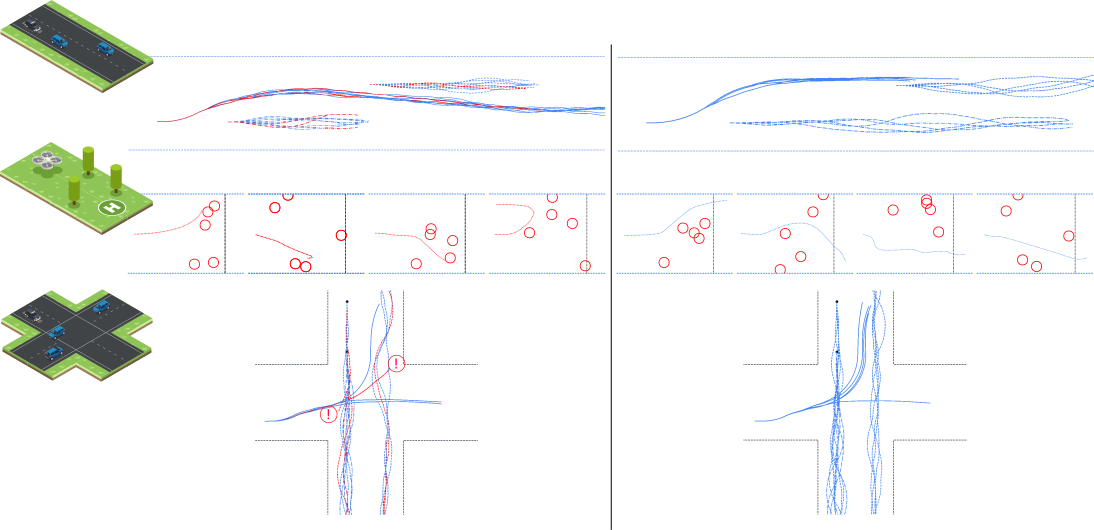
\includegraphics[width=\linewidth]{images/global_methods/repairs.png}
    \caption{Examples of failure cases (left) and repaired policies (right) generated using our method.}\label{global:fig:repairs}
\end{figure}

% Problem setup

% Research questions relevant to state of the art.

% Results

% How do our results compare to the state of the art? - Highlight overconfidence of gradient-only methods and poor solution quality of gradient-free methods.

\subsection{Discussion \& Limitations}

This chapter has presented the results of ongoing research demonstrating that:

\begin{enumerate}
    \item For problems with multiple local minima and poorly-conditioned gradients, an inference-based approach leads to more robust solution methods than an optimization-based approach.
    \item Optimization-as-Inference problems can be solved using either gradient-based or gradient-free methods, but gradient-based methods (enabled by automatic differentiation) perform much better on higher dimensional problems.
    \item The verification-guided design problem can be solved using a novel adversarial inference algorithm, a gradient-based version of which leads to faster convergence, better coverage of the failure space, and more robust designs.
\end{enumerate}

The results in this chapter, particularly regarding vision-based control, are preliminary; more work is needed to benchmark gradient-free and gradient-based inference methods against optimization methods on a range of robotics problems. In addition, although I have preliminary theoretical results that provide conditions under which gradient-based inference methods will work well (building on the results in~\cite{maSamplingCanBe2019}), more work is required to understand a) what features of a problem are required for this approach to work well (e.g. degree of smoothness, extent of discontinuity, etc.) and b) to develop runtime checks to determine whether a problem is well-suited for gradient-based inference.
